\label{gradience}

FIXME
%\begin{quote}
%Hence, a real solution to the problem of ``admissibility'' will not simply define a tripartite categorization of occurring, accidental gap, and inadmissible, but will define the `degree of admissibility' of each potential lexical matrix in such a way as to\ldots{}make numerous other distinctions of this sort (\emph{SPE}:416--417)
%\end{quote}
%
%\noindent
%The position that the well-formedness of nonce words is consistent the view of syntactic grammaticality taken in \emph{LSLT} and \emph{Aspects} \citep{LSLT,ASPECTS}, where it is claimed that different syntactic violations result in different degrees of ungrammaticality.
%
%Most recent discussions of the ``problem of admissibility'' focus on this cline of wellformedness as it is evidenced in wordlikeness tasks.
%
%\begin{quote}
%When native speakers are asked to judge made-up (nonce) words, their intuitions are rarely all-or-nothing. In the usual case, novel items fall along a gradient cline of acceptability. \citep[][9]{Albright2009a}
%
%In the particular domain of phonotactics gradient intuitions are pervasive: they have been found in every experiment that allowed participants to rate forms on a scale.
%\citep[][382]{Hayes2008a}
%
%\ldots{}when judgements are elicited in a controlled fashion from speakers, they always emerge as gradient, including all intermediate values. \citep[371]{Shademan2006} 
%\end{quote}
%
%\begin{quote}
%\ldots{}A defect of current grammatical acounts of phonotactics is that they render simple up-or-down decisions concerning well-formedness and cannot account for gradient judgements. \citep[371]{Shademan2006}
%\end{quote}

\section{What some wellformedness judgements might not be}

\begin{figure}
\centering
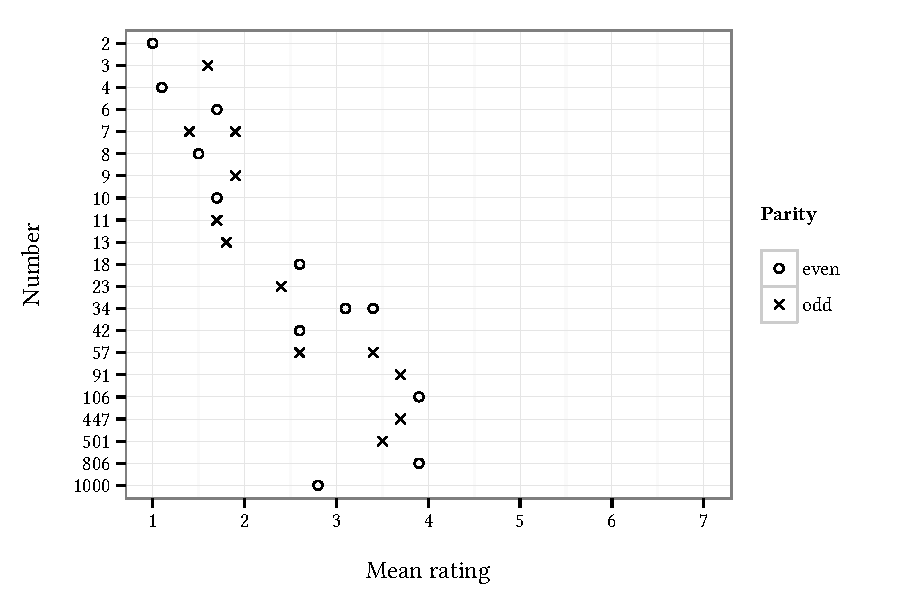
\includegraphics{agg.pdf}
\caption{Subjects freely use intermediate ratings when asked to rate how representative even and odd numbers were of ``even'' and ``odd'', respectively \citep{Armstrong1983}}
\label{agg}
\end{figure}

%The gradedness of a category cannot be observed. Scientists choose the granularity at which they observe. For example, a linguist may choose to record speakers' judgements on a 7-point scale, for example, or to use a forced binary choice between two minimally different items. The level of granularity at which the observations are made have consequences for how statistical inference over these observations should be performed, or for the theory of the \emph{task model}, the mechanism by which speakers perform the task, but it does not have any consequences for the \emph{theory} of phnotactics.

%\begin{quote}
%No integer seems to sit on the fence, undecided as to whether it is quite even, or perhaps a bit odd. No odd number seems odder than any other odd number. \citep[274]{Armstrong1983}
%\end{quote}

%\begin{quote}
%Some have responded to these findings very consistently, by asserting that the experimental findings are to be interpreted as before: that, psychologically speaking, odd numbers as well as birds and vegetables are graded concepts\ldots{} We reject this conclusion just because we could not explain how a person could compute with integers who believed that 7 was odder than 23. We assert confidently that the facts about subjects being able to compute and about their being able to give the definition of odd number, etc., are the more important, highly entrenched, facts we want to preserve and explain\ldots{} we ourselves are prepared to give up the seeming fact that some odd numbers appear, as shown by their behavior in certain experimental paradigms, to be odder than others\ldots{}we do not give it up by saying that it was no fact; rather, by saying it must have been a fact about something other than the structure of concepts. \citep[284]{Armstrong1983}
%\end{quote}

%\begin{quote}
%\ldots{}we hold that \emph{fruit} and \emph{odd number} have different structures, and yet we obtain the same experimental outcome for both. But if the same result is achieved regardless of the concept struture, then the experimental design is not pertinent to the determination of concept structure. \citep[284--5]{Armstrong1983}
%\end{quote}

\section{Evaluation}
\label{2evaluation}

There have been no serious attempts to evaluate categorical and gradient models of wordlikeness on an equal footing. This study represents a first attempt to fill this gap. It is not that categorical models have been ignored by the literature on wordlikeness modeling, but rather that they have not been compared. For instance, \citet{Hayes2008a}, who compare their gradient model of wordlikeness against a set of phonotactic constraints proposed by \citet{Clements1983}, transform the \citeauthor{Clements1983} constraints, many of which are exceptionless, into probabilities. While this is consistent with their claim that ``the ability to model gradient intuitions to be an important criterion for evaluating phonotactic models'' \citep[382]{Hayes2008a}, such a principle precludes any attempt to confirm or falsify the hypothesis that underlies it. 

It is unknown whether the intermediate ratings in gradient wordlikeness tasks are reliably predicted by the computational models that have been proposed. If some model poorly accounts for these intermediate ratings, it may be the case that the model is improperly specified, or it may indicate that a considerable amount of variance in wordlikeness ratings is not a product of the phonotactic system per se.

Imagine, alternatively, that wordlikeness judgements could be effectively modeled with a gross contrast between possible and impossible words. 

%[st] [bl]

\subsection{Materials}

This evaluation uses a large sample of three previously published studies on English wordlikeness comprising 125 subjects and 187 items. Two criteria were used to select these three studies. First, it was required that the stimuli be presented aurally so as to eliminate any possibility of orthographic effects. Secondly, the data must be sufficiently ``phonotactically diverse'': that is, it must include both items like \emph{blick} and \emph{bnick}. This excludes studies like that of \citet{Bailey2001}, in which few if any items contain gross phonotactic violations of the type represented by \emph{bnick}. The data is summarized in Table \ref{counts}.

\begin{table}
\centering
\begin{tabular}{l rrr}
\toprule
                           & subjects & items & trials \\
\midrule
\citeauthor{Albright2007}  & 68       & 40    & 2,720  \\
\citeauthor{Albright2003b} & 24       & 86    & 2,064  \\
\citeauthor{Scholes1966}   & 33       & 63    & 2,178  \\
\midrule
\textsc{Total}             & 125      & 187   & 6,962  \\
\bottomrule
\end{tabular}
\caption{Subject and item counts}
\label{counts}
\end{table}

\subsubsection{\citealt{Albright2007}}

\citet{Albright2007} administers a wordlikeness task in which 68 adult speakers rate 40 monosyllabic nonce words, presented aurally, on a 7-point Likert scale with endpoints labeled  ``completely impossible as an English word'' and ``would make a fine English word''. \citealt{Albright2007}'s study study is primarily concerned with the effects of different onset types (e.g., well-formed /bl/, marginal /bw/, unattested /bn, bd, bz/), and there is less diversity among the choice of rimes, none of which are obviously ill-formed.

\subsubsection{\citealt{Albright2003b} (norming experiment)}

\citet{Albright2003b} have 24 adult speakers rate 87 aurally presented monosyllabic nonce words on a 7-point Likert scale with endpoints labeled ``completely bizarre, impossible as an English word'' and ``completely normal, would make a fine English word''. This task was administered to establish phonotactic norms for a later nonce word inflection task. Their item [raɪf] is excluded in this study, since this is an actual word of English, \emph{rife}. \citet{Albright2009a} uses this data to evaluate several computational models of wordlikeness.

\subsubsection{\citealt{Scholes1966} (experiment 5)}

\citet{Scholes1966} conducts several wordlikeness tasks with 7th-grade students (approximately 12--13 years of age). The data used here is his experiment 5, in which 33 speakers provide a ``yes'' or ``no'' as to whether each of the 63 items, presented aurally, are ``likely to be usable as a word of English''. Like the study by \citet{Albright2007}, the focus was on onset well-formedness and there is minimal diversity in rime type. Two items, [klʌŋ] \emph{clung} and [bɹʌŋ] \emph{brung} (a dialectical past participle of \emph{bring}), are excluded here as actual words of English. \citet{Albright2009a} and \citet{Hayes2008a} also use this data for the purposes of model evaluation; following \citet{Frisch2000}, they use the proportion of ``yes'' responses for each item so as to derive a continuous measure of well-formedness.

\subsection{Method}

Models are evaluated by comparing their scores to the average rating of each word using four correlation statistics. \citet{Hayes2008a} evaluate their model using the Pearson $r$, a parametric measure of correlation. \citet{Stevens1946} argues that statistics of this type are inappropriate for analysis of Likert scale data, like those used by \citet{Albright2009a} and \citet{Albright2003b}. The reason is that this makes a \emph{linearity assumption}. That is, it assumes that nonce words rated ``1'' and  ``3'', for instance, are just as different as those ``4'' and a ``6''. A weaker assumption, more appropriate for Likert scale data, is the ``monotonicity assumption'': that ``1'' is less English-like than ``3'', which is less English-like than ``4'', and so on. However, it also has been claimed that $r$ is particularly robust to violations of the linearity assumption \citep[e.g.,][]{Havlicek1976}. Pearson $r$ is reported here, but no stance is taken on its appropriateness for this data.
%\citet{Jamieson2004}
\citeauthor{Hayes2008a} also report Spearman $\rho$; this statistic requires only the weaker assumption of monotonicity, but it is difficult to give a simple interpretation to the coefficient. Much easier to interpret are two non-parametric statistics, the Goodman-Kruskal $\gamma$ and the Kendall $\tau_b$ \citep{Noether1981}; a variant of the latter is used by \citet{Albright2009a}. These statistics are computed by comparing every model score/wordlikeness rating pair to every other: a comparison is counted as \emph{concordant} if the greater of the two model scores is the one associated with the greater of the two wordlikeness ratings (that is, the model ranks these two nonce words the in accordance with speakers' ratings), and as \emph{discordant} otherwise. $\gamma$ and $\tau_b$ differ in the treatment of ``ties'', pairs where either the model score or wordlikeness rating are identical. For $\gamma$, ties are ignored, and the coefficient is 

\begin{unlabeledexample}
$\gamma = \displaystyle\frac{c - d}{c + d}$
\end{unlabeledexample}

\noindent
where $c$ and $d$ represent the number of concordant and discordant pairs, respectively. The $\tau_b$ statistic uses a similar formula, but also incorporates a penalty for ties in model score which are not also paired with ties in wordlikeness ratings, or vis versa. 

\subsection{Models}

The nonce word stimuli from these three studies are scored automatically using four computational models. The first two models represent baselines for comparison to the latter two state-of-the-art gradient models. The scores for each model are provided in Appendix \ref{ratings}.

\subsubsection{Gross phonotactic violation}

A simple baseline is constructed by separating nonce words into those which contain a phonotactic violation and those which do not. As all nonce words here are monosyllabic, this task can be localized to two subcomponents of the syllable, the onset and the rime. This is not to imply that these are the only domains over which phonotactic violations might be stated, but there are prior claims that onset and rime are particularly important domains for stating phonotactic constraints (e.g., \citealt{Fudge1969}, \citealt{Kessler1997}, \citealt{Treiman2000}). Furthermore, these units are implicated by language games \citep{Treiman1983} and speech errors \citep{Fowler1993}, and adult speakers are adept at separating syllables into these units \citep{Treiman1986,Treiman1995}.

Operationalizing ``phonotactic violation'' is somewhat more difficult. The simplest possible mechanism is chosen here: an onset or rime is identified as well-formed if it occurs with non-zero frequency in a representative sample, and is identified as ill-formed otherwise. The sample is derived from those entries of the CMU pronunciation dictionary which occur at least once per million words in the SUBTLEX-US frequency norms, the latter though to be particualrly strongly correlated with behavioral measures \citep{Brysbaert2009}. These pronunciations are then syllabified, and individual syllables parsed into onset and rime, according to a process described in detail in Appendix \ref{syllabification}. This is not is not to imply that all unattested onsets or rimes should be regarded as ill-formed, or that all onsets or rimes with non-zero frequency in this data are well-formed. For instance, \citet{Albright2009a} judges [drEsp] to be an unobjectionable possible word of English, despite the total absense of [Esp] rimes in English, and similar observations have been made regarding English onsets \citep[e.g.,][]{Cairns1972,Moreton2002}.

In Figure \ref{boxplot}, wordlikeness ratings from the three studies are plotted according to this gross contrast. While there are a considerable number of outliers, there can be little doubt that the contrast is reflected in wordlikeness judgements in all three studies.

\begin{figure}
\centering
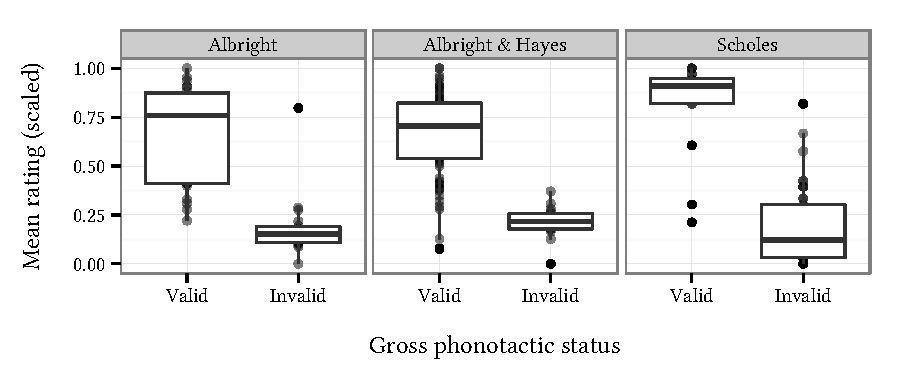
\includegraphics{boxplot.pdf}
\caption{Gross phonotactic status and item-averaged wordlikeness ratings}
\label{boxplot}
\end{figure}

\subsubsection{Lexical neighborhood density}

A second baseline is provided by measures of similarity to existing English words items, which has long been applied in the study of wordlikeness (e.g., \citealt{Greenberg1964}, \citealt{Ohala1986b}, \citealt{Shademan2006,Shademan2007}, \citealt{Vitevitch1998,Vitevitch1999a}). \citeauthor{LSLT} (\citeyear{LSLT}: 151, fn.~27) suggests that grammaticality judgements in general might be influenced by similarity to existing grammatical structures. \citet[417f.]{SPE} outline a similarity-based wordlikeness model. More recently, it has been observed (e.g., \citealt[51]{Coleman1997}, \citealt{Hay2004a}) that nonce words which flagrantly violate English sonority restrictions but which bear common affixes (e.g., *\emph{mrupation}) are rated highly English-like.

A wide variety of lexical similarity measures were considered, including a variant of including a variant of the Generalized Neighborhood model \citep{Bailey2001}, PLD20 \citep{Suarez2011}, and a set of measures provided by the Irvine Phonotactic Calculator \citep{Vaden2009}. The most reliable measure is also the most veneraable measure of lexical similarity: Coltheart's $N$ \citep{Coltheart1977}, which is defined as the number of words in some representative sample which can be changed into a target nonce word by a single insertion, deletion, or substitution of a phone. \citet{Greenberg1964} find a correlation between wordlikeness ratings and a variant of this measure which only counts words differing by a single substitution. This measure is plotted against ratings from the three studies in Figure \ref{neighborhood}, where it can be seen that it accounts for much of the variance in ratings.

\begin{figure}
\centering
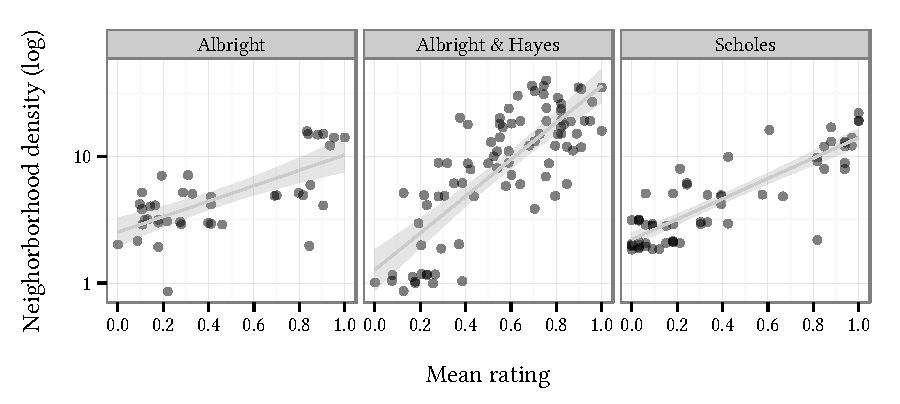
\includegraphics{neighborhood.pdf}
\caption{Correlation between neighborhood density and item-averaged wordlikeness ratings}
\label{neighborhood}
\end{figure}

While there is nothing inherently ``phonotactic'' about Coltheart's $N$, it indirectly incorporates much of the information present in the gross phonotactic baseline. Consider [blIk]: since there is nothing marked about any part of this nonce word, a ``neighbor'' might be found by modifying any phone: e.g., \emph{click}, \emph{brick}, \emph{bloke}, \emph{bliss}. However, since [bn] onsets are unattested in English, a neighbor of [bnIk] must somehow modify this cluster: this leaves only \emph{brick} and \emph{nick}. \citet{Frauenfelder1993} find that neighborhood density is also strongly correlated with measures like bigram probability.

\subsubsection{Segmental bigram probability}

Bigrams probabilities have been applied to model results of a number of psycholinguistic tasks \citep[e.g.,][]{Pitt1998,Vitevitch2005}, and \citet{Albright2009a} applies them as a model of wordlikeness judgements. The bigram probability of a sequence $ijk$, for instance, is:

\begin{unlabeledexample}
$\displaystyle \hat{p}(ijk) = p(i|\textrm{start}) \cdot p(j|i) \cdot p(k|j) \cdot p(\textrm{stop}|k)$
\end{unlabeledexample}

\noindent
That is, it is the product of sequence-initial $i$, the probability of $j$ following $i$, the probability of $k$ following $j$, and the probability of the sequence ending after $k$.

\citet{Albright2009a} compares two variants of this model, the first operating over segments, the second over sets of features. Unfortunately, the latter model is not described in sufficient detail to allow it to be implemented directly, and there is no publicly available implementation. However, \citeauthor{Albright2009a}'s evaluation, which includes the \citet{Scholes1966} and \citet{Albright2003b} data, finds an advantage for segmental bigrams. In implementing this model, it was found that a slight improvement could be made by preventing any phone-to-phone transition from have zero probability. This is accomplished by adding 1 to the count of every transition, a technique known as Laplace, or ``add one'', smoothing. As can be seen in Table \ref{bigramcomparison}, this results in a slight increase in the correlation between the scores from this model and wellformedness ratings. This smoothed segmental bigram score is adopted below. In Figure \ref{bigram}, it is plotted against wordlikeness ratings from the three studies.

\begin{table}
\centering
\begin{tabular}{l rrr}
\toprule
                         & features & segments & smoothing \\
\midrule
Pearson $r$              & {.711}   & {.742}   & \uline{.746} \\
Spearman $\rho$          & {.628}   & {.667}   & \uline{.699} \\
Goodman-Kruskal $\gamma$ & {.453}   & {.479}   & \uline{.502} \\
Kendall $\tau_{b}$       & {.448}   & {.473}   & \uline{.499} \\
\bottomrule
\end{tabular}
\caption{Correlation between item-averaged wordlikeness ratings for the \citet{Albright2003b} norming study and three variants of bigram probability; ``features'': featural bigram probability reported by \citet{Albright2009a}, ``segments'': segment bigram probability reported by \citet{Albright2009a}, ``smoothing'': segment bigram probabilities estimated using Laplace smoothing}
\label{bigramcomparison}
\end{table}

\begin{figure}
\centering
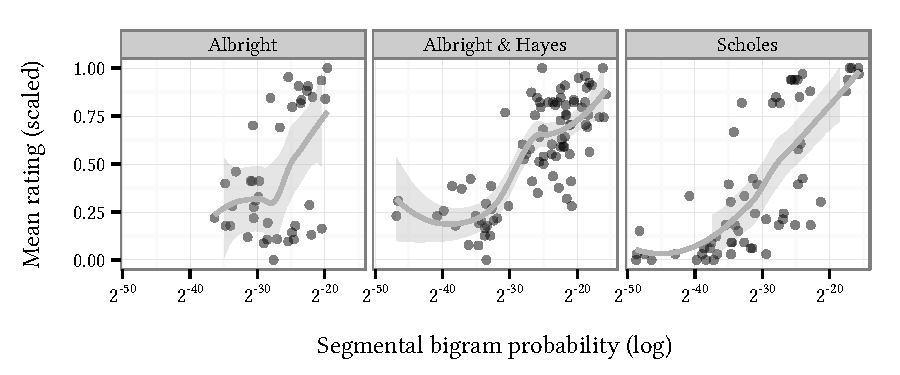
\includegraphics{bigram.pdf}
\caption{Correlation between segmental bigram score and item-averaged wordlikeness ratings}
\label{bigram}
\end{figure}

\subsubsection{Maximum entropy phonotactics}

\citet{Hayes2008a} propose a sophisticated model in which well-formedness is related to a probability distribution over phone sequences, estimated according to the principle of maximum entropy, or ``MaxEnt'' \citep[e.g.,][]{Goldwater2003,Jager2007}. \citeauthor{Hayes2008a} use a complex method to evaluate their model. First, they extract onset sequences from the CMU pronunciation dictionary which they use to train the model. The model is then used to score the onsets of the \citet{Scholes1966} nonce words. Then they compute a parameter for transforming their model scores so as to maximize the correlation between these transformed scores and wordlikeness ratings, then report the resulting corelation.\footnote{This is contrary to standard practices in natural language process, in that the data used for evaluation is also used to fit the model (namely, the transformation's parameter), and thus there is no indication that the model will generalize to new data. Consequently, no transformation is used here. This only has an effect on the Pearson $r$ coefficient, since they use a transformation that preserves monotonicity.}

An attempt was made to replicate the details of \citeauthor{Hayes2008a}'s evaluation as closely as is feasible: their software, model parameters, and feature specifications were all used. However, \citet{Albright2009a} finds that the maximum entropy model, training and testing only on onsets, does not generalize to the \citet{Albright2003b} data, presumably because of the considerable diversity of rimes in the latter data. Consequently, the model was trained to score whole words, not just onsets, using the subset of the CMU dictionary described above. Following the procedure of \citet{HayesInPress}, dictionary entries were syllabified and the resulting syllables were parsed into onset, nucleus, and coda, and a feature [$\pm$\textsc{Coda}] was added to contrast onset and coda consonants. Since the maximum entropy model, producing slightly different predictions on each run, the worst-performing of 10 runs is reported here, following \citet{Hayes2008a}. The resulting scores are plotted against wordlikeness ratings in Figure \ref{maxent}; it can be seen that the model assigns the highest possible score to large variety of nonce words, though many of these words appear to have a low rating. This suggests that the model is not robust enough to score whole words.

\begin{figure}
\centering
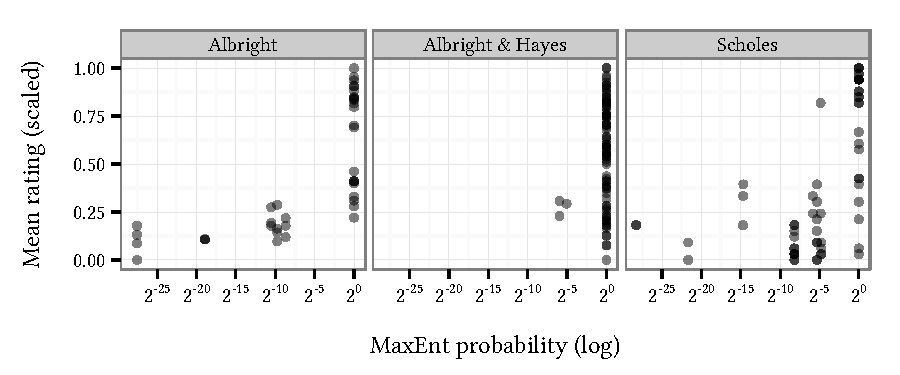
\includegraphics{maxent.pdf}
\caption{Correlation between MaxEnt score and item-averaged wordlikeness ratings}
\label{maxent}
\end{figure}

\subsection{Results}

Table \ref{scores} displays the full set of correlation coefficients, for each of the three data sets, and for each of the four models. For each pair of statistic and data set, the highest coefficient is underlined. The first observation is that in general, there is a positive correlation between model score and ratings in each pair. However, the two baselines, gross phonotactic status and neighborhood density, are by far the strongest models across statistics and and data, with gross phonotactic status performing the strongest under the Goodman-Kruskal $\gamma$ and on the \citet{Albright2007} data, and neighborhood density performing strongly under nearly all other statistics and data sets. 

\begin{table}
\centering
\begin{tabular}{l rrrr}
\toprule
                           & gross status & density ($N$) & bigram score & MaxEnt score \\
\midrule
Pearson $r$               \\
\midrule
\citeauthor{Albright2007}  & \uline{.725} & {.673}        & {.463}       & {.703} \\
\citeauthor{Albright2003b} & {.594}       & \uline{.793}  & {.746}       & {.208} \\
\citeauthor{Scholes1966}   & {.803}       & \uline{.855}  & {.737}       & {.534} \\
\midrule
Spearman $\rho$           \\
\midrule

\citeauthor{Albright2007}  & \uline{.819} & {.612}        & {.338}       & {.661} \\
\citeauthor{Albright2003b} & {.662}       & \uline{.739}  & {.699}       & {.389} \\
\citeauthor{Scholes1966}   & {.803}       & \uline{.817}  & {.794}       & {.575} \\
\midrule
Goodman-Kruskal $\gamma$  \\
\midrule
\citeauthor{Albright2007}  & \uline{.874} & {.488}        & {.246}       & {.849} \\
\citeauthor{Albright2003b} & \uline{.929} & {.574}        & {.502}       & {.606} \\
\citeauthor{Scholes1966}   & \uline{.907} & {.738}        & {.628}       & {.558} \\
\midrule
Kendall $\tau_{b}$        \\
\midrule
\citeauthor{Albright2007}  & {.666}       & {.450}        & {.245}       & \uline{.683} \\
\citeauthor{Albright2003b} & {.474}       & \uline{.558}  & {.499}       & {.159} \\
\citeauthor{Scholes1966}   & {.619}       & \uline{.671}  & {.614}       & {.484} \\
\bottomrule
\end{tabular}
\caption{Correlations between item-averaged wordlikeness ratings and model scores}
\label{scores}
\end{table}

\subsection{Discussion}

FIXME

\section{Conclusions}

FIXME

%%The primary result is that no gradient model reliably exceeds the accuracy of the binary baseline. Despite this, there are relatively strong correlations between the binary baseline and these gradient models (see Table \ref{bcor}). From the strong performance of the categorical model one can infer that the gradient models do not reliably predict intermediate ratings, or contrasts in ratings between words which are grouped together. To quantify this, the following method was used to estimate the residual contribution of the three gradient models once gross phonotactic violations are taken into account. Instead of calculating rank correlations directly on the model scores as in Table \ref{cor}, the model scores are mapped to ranks with the additional constraint that all ``valid'' stimuli be ranked above all ``invalid'' stimuli. The resulting ranks are used to compute new correlation statistics. Finally, the binary baseline correlation is subtracted from this number, so that the resulting value is the amount of improvement derived from augmenting the binary model with gradience. These difference numbers are shown in Table \ref{controlled}. In most cases, including the gradient models on top of the binary baseline produces a worse correlation than is obtained with the binary baseline alone.
%%
%%For $\tau_b$ and $\gamma$, the interpretation of this result is clear. The gradient models assign rankings to the sets of phonotactically valid and invalid clusters, respectively. For instance, the bigram model favors \emph{troog} [tɹuːɡ] over \emph{swach} [swætʃ], though neither contains any gross phonotactic violation. Similarly, the bigram model favors \emph{chwoop} [tʃwuːp] over \emph{zhrick} [ʒɹɪk], even though both contain ill-formed onsets. However, the majority of such predicted contrasts are not reflected in speakers' judgements; for instance, \emph{troog} is rated less English-like than \emph{swach} \citep{Greenberg1964}, contrary to the model predictions. This shows quite starkly that these models fail to reliably predict intermediate ratings.
%%
%%\subsection{The gradience hypothesis}
%%
%%This chapter has evaluated the axiom of gradience as a falsifiable alternative hypothesis. The surprising result is that virtually all of the apparent coverage of state-of-the-art gradient phonotactic models is simply a reflection of their ability to distinguish between the possible and the totally impossible; beyond this, they are unreliable. A trivial baseline, endowed with few abilities to project beyond the observed data, generally outperforms the state of the art. The projections made by the state-of-the-art gradient models are not like those made by speakers. It remains to be seen is whether any model can be put forth which accurately predicts these intermediate ratings.
%%
%%These result provide support for recent findings that speakers asked to perform gradient syntactic judgements produce responses closely corresponding to a widely recognized categorical grammatical/ungrammatical distinction \citep{Sprouse2007}.
%%
%%\subsection{Extensions to the binary baseline}
%%
%%The strong performance of the binary baseline should not be taken as evidence either that wordlikenesss judgements are binary, or that the binary baseline is a plausible model. The most serious limitation of this evaluation is the primitive nature of the binary baseline. The inability to generalization within onsets and rimes is a serious flaw, as is the assumption of independence of onset and rime. Regarding the rime, \citet{Borowsky1989} proposes a theory of possible rimes in English, which does make the correct prediction regarding the unattested but well-formed [ɛsp]. On the other hand, a cognitively plausible version of this model might need to entertain phonotactic generalizations that are larger than these units, since syllable-sized phonotactic generalizations have been proposed for English \citep[e.g.,][]{Berkley1994a,Berkley1994b,Coetzee2008b,Fudge1969}. 
%%
%%A possible further extension to the binary baseline would be the introduction of additional levels of wellformedness. While the evaluation has shown that current gradient models do not reliably identify intermediate wellformedness, it does seem possible to identify at least three levels of grammaticality: for instance, one might encode the intuition that \emph{zhlick} [ʒlɪk] is more English-like than \emph{bnick}, though both have unattested onsets. There are precedents for labeling certain attested words as phonotactically ``peripheral'' (see, e.g., the appendices in \citealt{Myers1987} and \citealt{Borowsky1989}); such words are regarded as lexical exceptions to language-general principles of syllabification. If this extends to nonce words, then an intermediate level of grammaticality could be assigned to ``possible'' but formally marked words. Another likely source of additional levels of grammaticality is the cumulative effect of multiple phonotactic violations. While, as \citet{Coleman1997} note, classical Optimality Theory predicts that a nonce word is as ill-formed as its worst deviation from syllable structure, it is possible to imagine that multiple phonotactic violations would result in greater degrees of ill-formedness. The bigram and maxent models make this prediction, as do many others \citep[e.g.,][]{Legendre1990,Levelt2000,Albright2008,Anttila2008a,Pater2009b} but despite this, there is still little data demonstrating cumulative effects in wordlikeness tasks.
%%
%%\subsection{Language acquisition}
%%
%%The weak empirical status of gradient phonotactic knowledge as reflected in adults has rammifications for language acquisition under the hypothesis that that infants acquiring language deploy the same representations as adults \citep[e.g.,][]{Macnamara1982,Pinker1984,Crain1991,Carey1995,deVilliers2001,Legate2007}. Gradient wordlikeness judgements in adults would provide support for claims that infants recognize statistical(inherently gradient) dependencies between segments \citep{Jusczyk1994} and use these to segment words \citep{Saffran1996}. An emerging consensus suggests, however, that infants attend to transitional probabilities primarily in the absence of grammatical cues \citep{Gambell2005,Hohne1994,Johnson2001,Jusczyk1999c,Lignos2012b,Mattys2001a,Shukla2007,Lew-Williams2012}. The vacuous nature of current evidence for gradient phonotactic knowledge in adults further weakens any hypothesis that would link statistical learning in infants to adults' behaviors.

%% Hayes2000
% 
% Bard1996
% 
% Koo2009
% 
% 

% 
% Warker2006
% 
% Massaro1983
% 
% Rusaw2009

%%do not explicitly state why this data is relevant to the construction of models of wordlikeness. Presumably, these authors believe that these patterns of judgements demonstrate that wordlikeness, as an internal state, is gradient simply because subjects make use of intermediate degrees of wordlikeness in judgement tasks. This proposition, generalized below, is ``naïve'' not because it lacks sophistication, but because it is rooted in a belief in naïve realism, a philosophy which holds that perception provides a relatively direct picture of the nature of the world, an influential view in the cognitive sciences in general (see \citealt{Fodor1981a} for a critique).

%%\citeauthor{Chomsky1965} were not the first to consider the notion of possible and impossible words. Their primary contribution is that their mentalist perspective: they recognize that naïve speakers effortlessly acquire language-specific generalizations about possible and impossible words and can report them without any explicit training.
 
%%However, not all early literature is concerned with gradience. \citet[31]{Vogt1954}, for instance, recognizes that the taxonomic phoneme is insufficient to account for many wordlikeness contrasts. \citeauthor{Vogt1954} observes that allophony may account for the absence of certain phone sequences, but it does not provide a suitable explanation for the absence of initial [bn] in English, nor does it make correct predictions about the surface realization of an underlying initial /bn/. \citeauthor{Vogt1954} concludes that additional grammatical machinery will be needed to account for possible and impossible words. 
 
%%Most relevant to the question at hand, \citet{Frisch2000} and \citet{Vitevitch1997} find that speakers' wordlikeness ratings of multisyllabic words are correlated wtih the positional probailities of the constituent syllables. Unfortunately, none of these researchers make any effort to eliminate the possibility that the low positional probability stimuli are ``impossible'' words of English. In fact, 

%Chapter \ref{clusters} argues
%that many of the stimuli used by \citeauthor{Frisch2000} and \citeauthor{Vitevitch1997} contain illicit word-medial consonant clusters. While \citeauthor{Vitevitch1997} neither control nor manipulate the well-formedness of medial clusters, in a post-hoc test they consider a probabilistic measure of cluster well-formedness, which reveals that cluster well-formedness is correlated with syllable-internal positional probabilities and wordlikeness judgements, but \citeauthor{Vitevitch1997} ultimately conclude this cannot explain all the variation in wordlikeness. 
 
%Using the head-term preference paradigm, \citet{Jusczyk1993b} and \citet{Friederici1993} find that typically-developing children as young as 9 months of age distinguish between nonce words which are and are not phonotactically valid in their target language. \citet{Jusczyk1994} report that 9-month-old children acquiring English also show preferences for nonce words with high positional probability over those with low positional probability. Faciliatory effects of positional probability (i.e., shorter latencies) are reported for other nonce word tasks conducted with adults, including single-word shadowing \citep{Vitevitch1997,Vitevitch1998}, same/different judgements \citep{Vitevitch1999a,Luce2001,Lipinski2005,Vitevitch2005}, and lexical decision \citep{Pylkkanen2002a}.
  
%%The aforementioned studies all conclude that the gradient measure of positional probability correlates with behavioral results. As the flaws of the \citet{Vitevitch1997} study demonstrate, the aforementioned studies do little to tease apart the gradient and categorical aspects of phonotactics. More generally, they do little to distinguish between positional probability and closely correlated measures like bigram probability (see \S\ref{bigram} below) or neighborhood density, since these studies carefully select stimuli which either have high or low values for all of positional probability, bigram probablility, and neighborhood density. This is particularly troublesome given that no justification has ever been given for the positional probability measure in the first place; it appears to have been created \emph{ex nihilo}; in contrast, the effects of neighborhood density in various psycholinguistic tasks are emergent properties of many models of speech production \citep[e.g.,][]{Luce1998,Luce2000} and perception \citep{Marslen-Wilson1984,Marslen-Wilson1987,McClelland1986,Norris1994,Norris2000}. 
